\documentclass[11pt]{article}

%%%%%%%%%%%%%%%%%%%%%%%%%%%%%%%%%%%%%%%%%%%%%%%%%%%%%%%%%%%%%%%%%%%%%%%%%%%%%%%%
% packages
%%%%%%%%%%%%%%%%%%%%%%%%%%%%%%%%%%%%%%%%%%%%%%%%%%%%%%%%%%%%%%%%%%%%%%%%%%%%%%%%

\usepackage{coling2020}
\usepackage{times}
\usepackage{url}
\usepackage{latexsym}
\usepackage{amsmath,amsfonts}
\usepackage{graphicx}
\usepackage{bbm}
\usepackage{hyperref}
\usepackage{booktabs}
\hypersetup{
  colorlinks   = true, %Colours links instead of ugly boxes
  urlcolor     = blue, %Colour for external hyperlinks
  linkcolor    = blue, %Colour of internal links
  citecolor    = blue  %Colour of citations
}

%
%%%%%%%%%%%%%%%%%%%%%%%%%%%%%%%%%%%%%%%%%%%%%%%%%%%%%%%%%%%%%%%%%%%%%%%%%%%%%%%%
% latex functions
%%%%%%%%%%%%%%%%%%%%%%%%%%%%%%%%%%%%%%%%%%%%%%%%%%%%%%%%%%%%%%%%%%%%%%%%%%%%%%%%

\newcommand{\ltwo}[1]{\lVert{#1}\rVert}
\newcommand{\indicator}[1]{\mathbbm{1}\!\left[{#1}\right]}
\newcommand{\R}{\mathbb R}
\newcommand{\TEXT}{\texttt{text}}

\newcommand{\defn}[1]{\emph{{#1}}}
\newcommand{\fixme}[1]{\textbf{FIXME: {#1}}}

\DeclareMathOperator*{\argmax}{arg\,max}
\DeclareMathOperator*{\argmin}{arg\,min}
\DeclareMathOperator{\acc}{acc}
\DeclareMathOperator{\none}{\texttt{None}}
\DeclareMathOperator{\dataset}{\texttt{RTArticles}}


%%%%%%%%%%%%%%%%%%%%%%%%%%%%%%%%%%%%%%%%%%%%%%%%%%%%%%%%%%%%%%%%%%%%%%%%%%%%%%%%
% paper configuration
%%%%%%%%%%%%%%%%%%%%%%%%%%%%%%%%%%%%%%%%%%%%%%%%%%%%%%%%%%%%%%%%%%%%%%%%%%%%%%%%

%\setlength\titlebox{5cm}
%\colingfinalcopy % Uncomment this line for the final submission

% You can expand the titlebox if you need extra space
% to show all the authors. Please do not make the titlebox
% smaller than 5cm (the original size); we will check this
% in the camera-ready version and ask you to change it back.


\title{Instructions for COLING-2020 Proceedings}

\author{First Author \\
  Affiliation / Address line 1 \\
  Affiliation / Address line 2 \\
  Affiliation / Address line 3 \\
  {\tt email@domain} \\\And
  Second Author \\
  Affiliation / Address line 1 \\
  Affiliation / Address line 2 \\
  Affiliation / Address line 3 \\
  {\tt email@domain} \\}

\date{}

%%%%%%%%%%%%%%%%%%%%%%%%%%%%%%%%%%%%%%%%%%%%%%%%%%%%%%%%%%%%%%%%%%%%%%%%%%%%%%%%
% document text
%%%%%%%%%%%%%%%%%%%%%%%%%%%%%%%%%%%%%%%%%%%%%%%%%%%%%%%%%%%%%%%%%%%%%%%%%%%%%%%%

\begin{document}
\maketitle
\begin{abstract}
\end{abstract}

%
% The following footnote without marker is needed for the camera-ready
% version of the paper.
% Comment out the instructions (first text) and uncomment the 8 lines
% under "final paper" for your variant of English.
% 
\blfootnote{
    %
    % for review submission
    %
    \hspace{-0.65cm}  % space normally used by the marker
    Place licence statement here for the camera-ready version. 
    %
    % % final paper: en-uk version 
    %
    % \hspace{-0.65cm}  % space normally used by the marker
    % This work is licensed under a Creative Commons 
    % Attribution 4.0 International Licence.
    % Licence details:
    % \url{http://creativecommons.org/licenses/by/4.0/}.
    % 
    % % final paper: en-us version 
    %
    % \hspace{-0.65cm}  % space normally used by the marker
    % This work is licensed under a Creative Commons 
    % Attribution 4.0 International License.
    % License details:
    % \url{http://creativecommons.org/licenses/by/4.0/}.
}

\section{Introduction}
\label{sec:intro}


Research on text retrieval tasks has been pivotal to the Natural Language Processing field, but this work has been focused on singular language comparisons (CITATION NEEDED). This paper will both develop and implement the techniques needed to analyze retrieval tasks in the multilingual case. We examined the Russia Today (RT) newspaper, which is an official newspaper of the Russian government, and is one of Russia's primary tools for public diplomacy. RT publishes articles written in the Russian language that target the Russian diaspora, but RT also publishes articles in Arabic, English, French, German and Spanish that target a non-Russian audience. However, not all articles published in RT are translated into each language. Since the editors only publish articles in a specific language if those articles will be of interest to speakers of that language, we are able to directly examine these differences in content between languages. 

%Previous work has studied the political bias in English-only RT articles with respect to military expansion in the arctic \cite{bushue2015framing} and the Syrian Civil War \cite{wasuwong2016study}.
%Wikipedia \cite{hale2014multilinguals,hecht2009measuring,hecht2010tower}
%\fixme{VOA/BBC \cite{rampal1990credibility}}

\subsection{Contributions}

This paper has 4 distinct contributions.

\begin{enumerate}
    \item 
        We introduce the Missing Content Task for information retrieval which is a generalization of the Bitext Retrieval Task to the missing data regime.
    \item 
        We provide the first empirical comparison of the multilingual BERT and USE models on both the Bitext Retrieval and Missing Content tasks.
    \item 
        We introduce the $\dataset$ dataset for the Missing Content task.
        This dataset contains newspaper articles published in RT in six different languages.
    \item 
        We use the results of the Missing Content task on $\dataset$ to provide the first multilingual analysis of the publication biases of Russian state-owned media.
\end{enumerate}

\section{Method Overview}
\label{sec:method}

In this section we introduce the \defn{Missing Content} (MC) Task as a generalization of the \defn{Bitext Retrieval} (BR) Task to the missing data regime.
BR is a standard task in multilingual document retrieval that is used to measure the quality of multilingual document embeddings, and it has seen significant recent study \cite{}.
We begin by introducing our notation and formally describing the BR task.
Then we formally define our MC generalization.

\subsection{Bitext Retrieval (BR) Task}

We are given a corpus of $n$ text documents,
and each document has a translation into into several different languages.
Let $C_\ell = \{ c_\ell^1, c_\ell^2, ..., c_\ell^{n} \}$ be the subcorpus for language $\ell$,
where $c_\ell^i$ is the $i$th document in the corpus translated into language $\ell$.
In particular, for any document index $i$ and any two languages $\ell$ and $\ell'$,
the documents $c_{\ell}^i$ and $c_{\ell'}^i$ contain the same text translated into different languages.

The goal of the \defn{Bitext Retrieval} (BR) Task is to use the document corpus for machine translation.
That is, given a source document $\gamma\in C_\ell$ and target language $\ell'$,
the goal is to find the document $\gamma' \in C_{\ell'}$ that is a translation of $\gamma$.
This problem is difficult because the translation function cannot access the document indices and must operate only on the document text.\footnote{%
In a real problem, the document indices $i$ would be latent parameters of the data,
and the input corpus would be presented in unsorted order.
We present the datasets in sorted order with an explicit index for notational convenience only.}

The standard solution to the BR Task uses document embeddings.
Let $f : \TEXT \to \R^d$ be a function that embeds text into a $d$-dimensional vector space;
that is, it converts any document $c_\ell^i$ into a vector. 
A good embedding function function should satisfy two properties.
First, it should embed similar documents into similar vectors regardless of the documents' languages.
That is, $f$ should satisfy
\begin{equation}
    \ltwo{f(c_{\ell}^i) - f(c_{\ell'}^i)} \approx 0 ~\text{for all}~ \ell,\ell',i
    .
\end{equation}
Second, $f$ should embed dissimilar documents into dissimilar vectors.
That is, it should satisfy
\begin{equation}
    \ltwo{f(c_{\ell}^i) - f(c_{\ell'}^j)} >\!\!> 0 ~\text{for all}~ \ell,\ell',i\ne j
    .
\end{equation}
In our experiments, we use the multilingual BERT \cite{} and USE \cite{} models which are known to satisfy these properties.

To solve the BR Task using document embeddings, we first compute the distance matrix $M$ defined by 
\begin{equation}
    \label{eq:M}
    M_{ij} = \ltwo{ f (c_{\ell}^i) - f(c_{\ell'}^j ) }.
\end{equation}
Then for each document $i$ in language $\ell$, we compute its translation by finding the document in language $\ell'$ with minimum distance.
That is, we compute
\begin{equation}
    \label{eq:jhat}
    \hat j(i) = \argmin_{j\in[n]} M_{ij}
\end{equation}
and set the translation of $c_{\ell}^i$ to be $c_{\ell'}^{\hat j(i)}$.
If $\hat j(i) = i$, then we say the translation is correct,
otherwise we say the translation is incorrect.
The overall accuracy of the BR Task is given by
\begin{equation}
    \acc_{BR}(\ell,\ell') = \frac 1 n \sum_{i=1}^n \indicator{\hat j(i) = i}
    .
\end{equation}

\subsection{Missing Content (MC) Task}

The \defn{Missing Content} (MC) Task is the natural extension of the BR Task to the missing data setting.
In particular, the MC Task allows each of the input $c_\ell^i$ variables to be either a translation of document $i$ into language $\ell$ or the special value $\none$ if no such translation is provided.
The goal of the MC Task is then the same as the goal of the BR Task:
Take an input document $\gamma\in C_\ell$ and target language $\ell'$,
and output the corresponding value $\gamma' \in C_{\ell'}$.
In the BR Task, the output $\gamma'$ is guaranteed to be a document,
but in the MC Task, the output $\gamma'$ may also be the special token $\none$ if no suitable translation is found.

We propose to solve the MC task using a natural generalization of the standard BR algorithm above.
Calculate the $M$ matrix as
\begin{equation}
    M_{ij} = 
    \begin{cases}
        \infty & \text{if}~ c_{\ell}^i = \none ~\text{or}~ c_{\ell'}^j=\none \\
        \ltwo{ f (c_{\ell}^i) - f(c_{\ell'}^j ) } & \text{otherwise}
    \end{cases}
\end{equation}
and calculate
\begin{equation}
    \hat j(i) = 
    \begin{cases}
        \argmin_{j\in[n]} M_{ij} & \text{if}~ \min_{j\in[n]} M_{ij} < \tau \\
        \none & \text{otherwise}
    \end{cases}
    ,
\end{equation}
where $\tau$ is a threshold hyperparameter that controls the trade-off between the precision versus recall of our algorithm.

The generalization of the accuracy to the MC Task is given by
\begin{equation}
    \acc_{MC}(\ell,\ell') = \frac 1 n \sum_{i=1}^n \indicator{\hat j(i) = i ~\text{or}~ (\hat j(i) = \none ~\text{and}~ c_\ell^i = \none) }
    .
\end{equation}

The choice of $\tau$ is obviously of critical importance,
and a logical choice of $\tau$ is one that maximizes the accuracy on a held-out validation set.

\fixme{add a discussion of how tau effects the precision/recall of the model.}

\section{Experiments}
\label{sec:experiments}
\subsection{The Datasets}
The United Nations Parallel Corpus \cite{NEED CITATION} is composed of the UN's official public records, hand translated by professional translators into 6 languages: Arabic, English, Spanish, French, Russian, and Chinese. Since, the raw dataset is 65GBs decompressed, we create a subset of the raw dataset due to computation constraints (Corpus subset). We reduce the length of every text file from 13,000,000 lines(FIGURE OUT EXACT NUMBER) to 100,000 lines. Then generate a list of 100,000 uniformly random indices and strip out those indices from every document, ensuring every line in the Corpus Subset matches correctly across all 6 languages. 

From the Corpus subset we create another subset (MC Corpus subset) that has varying numbers of lines removed from the texts. First, fix a 100,000 random values between 0 and 1, then for any given missing content rate we check if the corresponding random value is less than or equal to the given missing content rate and remove the line the input document, otherwise, continue to the next line. This process produces an input document that can have any percentage of missing data. 

The Russia Today dataset (RT) contains the newspaper titles for the 6 languages published by Russia Today: English, Russian, German, French, Arabic, and Spanish. "Russia Today" is an official newspaper of the Russian government, and is one of Russia's primary tools for public diplomacy. We can see in Figure x that the amount of articles published in each language varies considerably. This provides a perfect dataset for the Missing Content Task where we can examine the relationship between which languages each article is published in. 

\fixme{Add figure about number of lines in each language}

\subsection{Model Choices}
For Sentence translation, we test both the BERT\cite{Citation Needed} and the Universal Sentence Encoder (USE) \cite{Citation Needed}. Both models are commonly used in research, but often for differing tasks \cite{Citation Needed}. Directly comparing the two models, BERT supports more languages than USE, 104 to 16 respectively. However, when both models are tested on the Corpus Subset (FIGURE 1) USE clearly outperforms BERT. The large accuracy disparity is likely, in part, due to how each model is trained. BERT is trained on two main tasks, Masked Language and Next Sentence Prediction \cite{Citation Needed}. On the other hand, USE is primarily trained on similarity between sentence pairs \cite{Citation Needed}, which is exactly the task preformed in our experiments. Since USE supports all the languages in both the Corpus Subset and RT there is no downside to choosing USE over BERT, thus we use USE in the Missing Content Tasks. 


\subsection{Corpus Subset Experiments}
A precursor to the Missing Content Task requires that the our sentence translation model is able to accurately compare information in multiple languages. To verify that the USE is suitable for the Missing Content Task we replicate the experiments done by Google \cite{Citation Needed}, instead testing on the introduced Corpus Subset. The results of the Bitext Retrieval task can be seen in Figure 1. The USE model preforms exceptionable on the Corpus Susbset, which implies that the Missing Content Task will contain minimal error due to inaccurate language translations.  



% \fixme{How we obtained the accuracies? Is that not already stated in the math portion? Need help here, not sure what to write, or is this even a needed section anymore?}

% Take two texts as input, then utilize the Universal Sentence Encoder (USE) (Citation Needed) to embed each line from the texts into a $512$ dimensional vector space. This vector space contains both the semantic and literal meaning of each of the sentences irrespective of the input language. Thus, we are able to compare text embeddings from different languages. While there are several models that can generate word embeddings we found that the USE model was extremely accurate as seen in Figure 1. For testing purposes, we utilize the United Nations Parallel Corpus Dataset (UN Dataset) as it contains texts in 6 different languages that are hand translated by linguists. Since, we know that every line in the Dataset should have near identical word embeddings we can simply calculate a matrix of all possible L2 distances between each line for a given language comparison. Then we verify that the minimum distances in each row of the matrix indeed correspond to the correct line number. These accuraices for each language pair are shown in Figure 1. 


\subsection{MC Corpus Subset Experiments}
After replicating the accuracy of the USE, we test the proposed Missing Content task on the MC Corpus subset to both prove that the Missing Content Task is solvable and to examine how varying $\tau$ affects the trade-off between precision and recall. The results of our testing is shown in Figure 2, displaying the ROC curves of 9 different missing content rates. Every ROC curve shows that there is little trade-off between precision and recall and in particular, even when 90 percent of the data is removed, the USE is still able to accurately predict when the data is missing. Thus, when using the USE, we can minimize any error in the Missing Content task due to language translation mistakes. Furthermore, we prove that their exist environments where the Missing Content task is a solvable. Since the Missing Content task solvable, we are able to propose more than a new benchmarking technique, we are able to extract meaningful analysis about datasets with missing information. 

% Once we determined that the USE model had high enough accuracy, we test the proposed Missing Content task on the MC Corpus subset for varying $\tau$ threshold values. Figure 2 provides an example language comparison ROC curves for varying missing data rates. 

% We show the Missing Content task is solvable by replicating pervious USE experiements done by google on Corpus Subset with very good results. 

% This is extremely important because we can guranteee that the Missing Content Task is solvable, for the languages in the Corpus subset. 

% This extends the missing content task from simply a new cool technique to further benchmarks multilingual encoders towards actually being able to extract usfull information about datasets with missing content. 


% Thus we can minimize error in Missing content task due to model translation deficiencies  


% notice that even when 90 percent of the data is missing the ROC curves are still good, which implies that the missing Content task can be done even with datasets where some languages have far larger amounts of data than others. 


% \fixme{Specifics of why these ROC curves are important}  


\subsection{RT Experiments}
The application of the MC task to datasets that originally contain unknown information can be much more difficult. While the UN Dataset always has a known value for every line in the texts, for the interesting datasets, there likely will be no such baseline to precisely choose an appropriate $\tau$. Consider Russia Today (RT), where there is no easy method to guarantee if a given article in one language exists in the comparison language or is in actuality missing. Thus, the choice of $\tau$ for any particular run will have a large effect on the output of the model. To examine the effect a particular $\tau$ has on the model, we graph the Found Content rate for varying $\tau$ as well as differing decision criteria. The base decision criteria is, for every line in document 1, return "found" if a non zero number of L2 distances between every line in document 2 is less than the particular $\tau$. However, while this approach technically is correct, it inadvertently omits possible insights into the distribution of these matching lines. To fully describe the comparison documents, we simply vary the described decision criteria. 

Let $\tau_0,\tau_1,\tau_2...\tau_i \in (a,b): a,b \in \mathbb{R}$.
Let $k_0,k_1,k_2...k_j$ be the distance from line $1,2,3...i$ in document 1 to line $1,2,3...j$ in document 2. 
Let $\gamma$ be the $\sum \forall k$ $:k<\tau$.
Let $n \in [\alpha,\beta]$ $:\alpha,\beta\in \mathbb{I}$. 
Then $\forall$ lines in document 1 the decision criteria is given by:

\begin{center}
\[   \left\{
\begin{array}{ll}
      Found & \gamma=n \\
      Missing & otherwise \\
\end{array} 
\right. \]
\end{center}    
For every $n$ now obtain a graph of the Found Content rate $\forall \tau \in (a,b)$. For illustration purposes we fix $\n \in [0,9]$, see Figure 3.    

\fixme{Why we care:
provides another way models can be tested vs each other
can specifically identify when and where content is missing from two comparison documents 
}

\fixme{Add section about an example of an interesting missing content as well as consider adding the TSNE-figure}

   

\begin{figure}
    \centering
    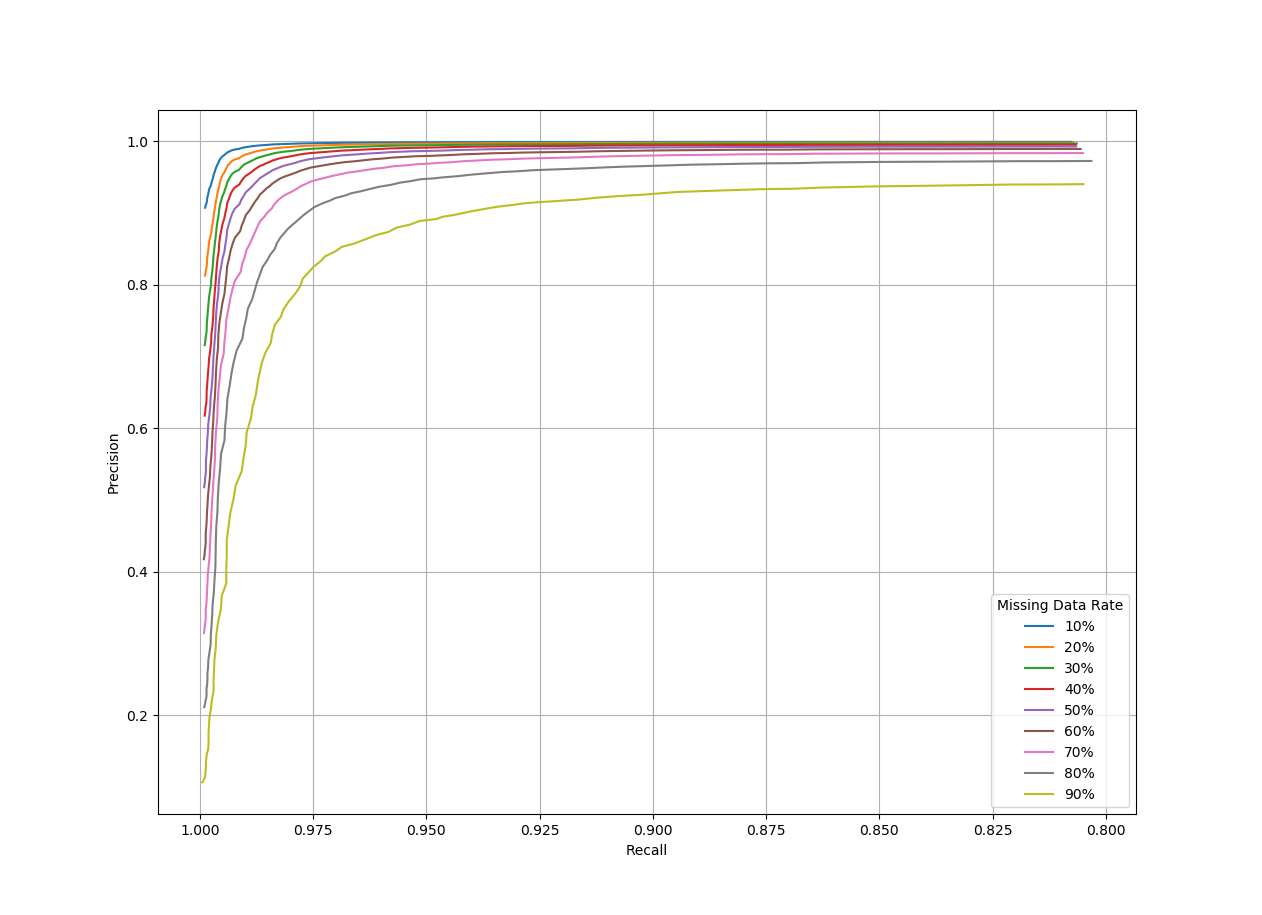
\includegraphics[height=2in]{recall_precision_first_test_zoomed.png}
    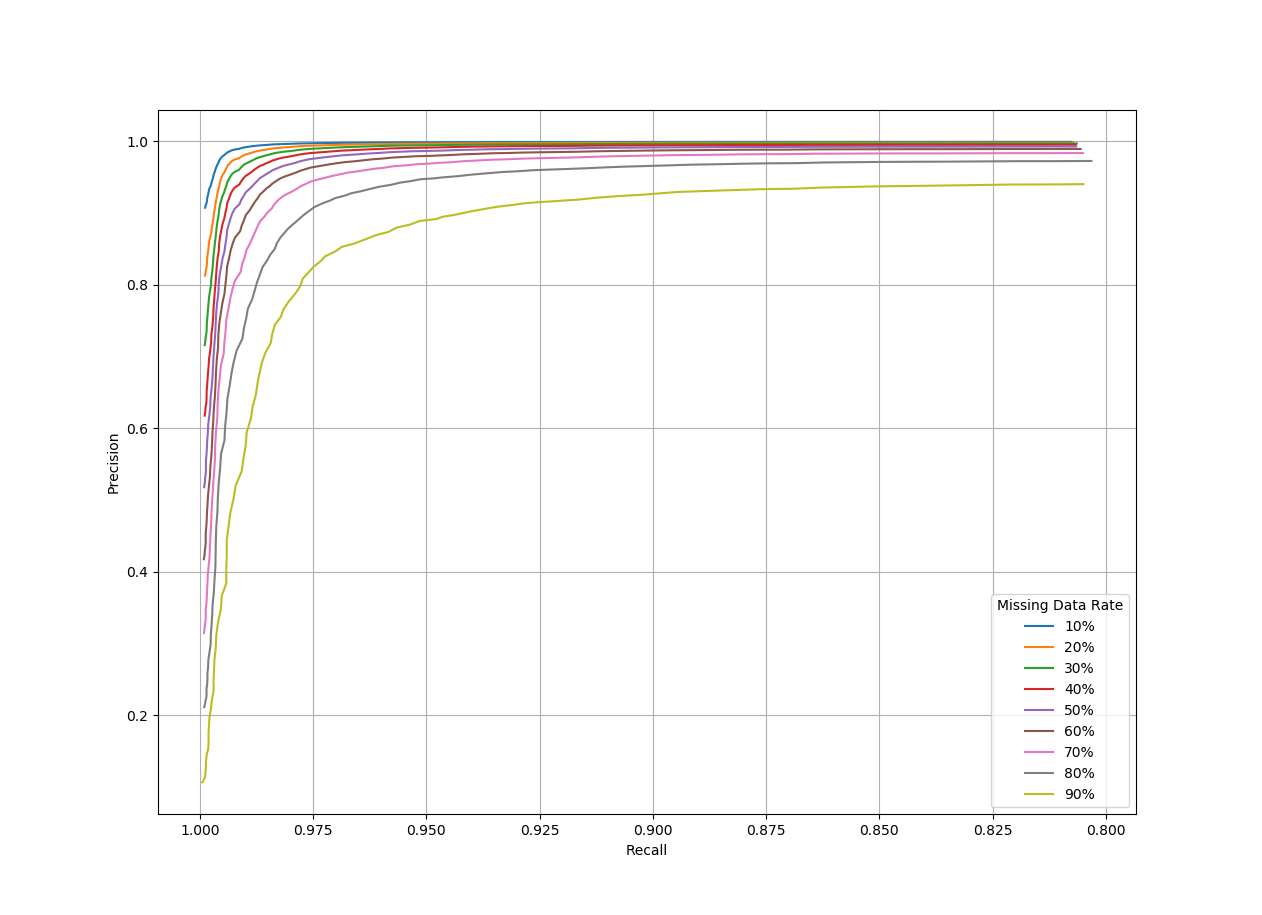
\includegraphics[height=2in]{recall_precision_first_test_zoomed.png}
    \caption{
        Plot of the $M_{ij}$ values used to determine the threshold $\tau$ and a ROC curve.
        To start with, you should plot the distribution of diagonal and off-diagonal points on the same plot, but in different colors.
        The easiest way to plot an empirical distribution is using the empirical CDF,
        but a histogram is a bit easier to interpret intuitively.
        There should be a large separation between these two distributions,
        and the optimal $\tau$ value is intuitively the location that provides the best separation between these two distributions.
    }
\end{figure}

\begin{table}
    \centering
    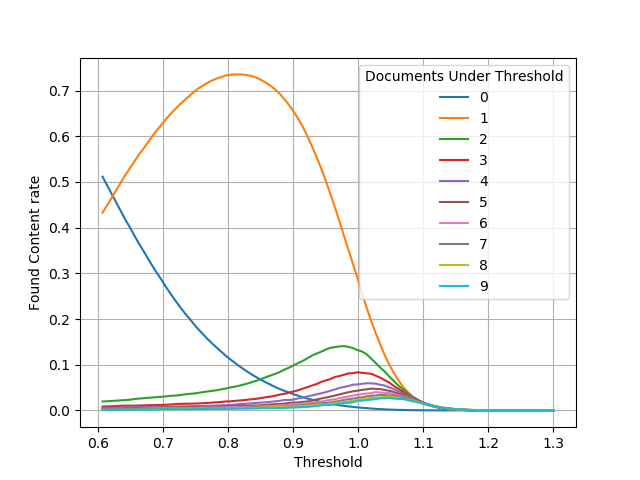
\includegraphics[height=2in]{fr_en_un_equal_to.png}
    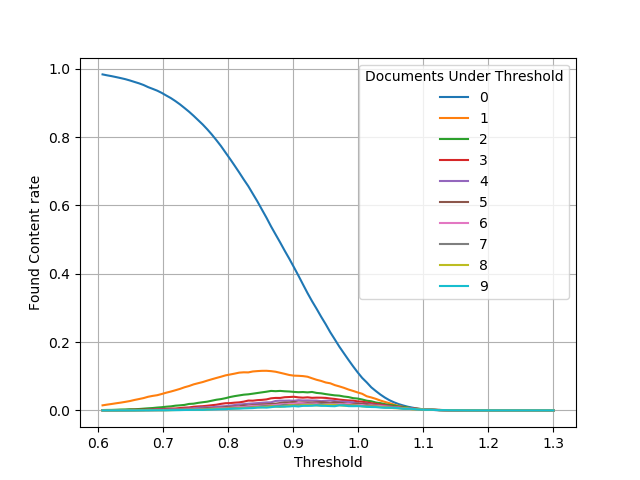
\includegraphics[height=2in]{fr_en_equal_to.png}
    \caption{RT and UN missing Content example, Left:UN, Right:RT}
\end{table}

\begin{table}
    \centering
    \includegraphics[height=2in]{example-image-a}
    \caption{Example article headlines in multiple languages}
\end{table}

\begin{table}
    \centering
    \includegraphics[height=2in]{example-image-a}
    \caption{Table similar to UN tables but for the Article dataset}
\end{table}

\begin{figure}
    \centering
    \includegraphics[height=2in]{example-image-a}
    \caption{Visualization of the document graph for the Article dataset}
\end{figure}

\section{Related Work}
\label{sec:related}
% \begin{table}
%     \begin{tabular}{llllll}
%     \centering
% \toprule
% {} &    es &    ru &    fr &    zh &    en \\
% \midrule
% es &  100\% &   63\% &   74\% &   22\% &   74\% \\
% ru &   70\% &  100\% &   78\% &   27\% &   56\% \\
% fr &   80\% &   67\% &  100\% &   26\% &   81\% \\
% zh &   28\% &   27\% &   33\% &  100\% &   32\% \\
% en &   55\% &   37\% &   65\% &   16\% &  100\% \\
% \bottomrule
%     \caption{This is the table you've been creating for the UN dataset.}
% \end{tabular}

% \end{table}



% \subsection{Ben}

% Very similar to what we want to do: \cite{rupnik2016news,miranda2018multilingual,wang2018estimation,germann2019scalable,seki2018exploring,seki2020cross,linger2020batch}

% Brexit case study: \cite{peterlin2019detecting}

% Also similar, but involving search terms; probably just good for citations and not techniques: \cite{rupnik2016news}

% Multilingual BERT:

% \cite{K2020Cross-Lingual}

% \cite{pires2019multilingual}

% More multilingual models non-BERT from google:

% https://ai.googleblog.com/2019/07/multilingual-universal-sentence-encoder.html

% https://arxiv.org/abs/1807.11906
% https://arxiv.org/abs/1810.12836
% https://arxiv.org/abs/1902.08564
% https://arxiv.org/abs/1906.08401
% https://arxiv.org/abs/1907.04307

% Old survey but good on non deep learning techniques of the era: \cite{oard1998survey}.

% \section{Discussion}
% \label{sec:discussion}


% \bibliographystyle{coling}
% \bibliography{main}

\end{document}
